\documentclass[1p]{elsarticle_modified}
%\bibliographystyle{elsarticle-num}

%\usepackage[colorlinks]{hyperref}
%\usepackage{abbrmath_seonhwa} %\Abb, \Ascr, \Acal ,\Abf, \Afrak
\usepackage{amsfonts}
\usepackage{amssymb}
\usepackage{amsmath}
\usepackage{amsthm}
\usepackage{scalefnt}
\usepackage{amsbsy}
\usepackage{kotex}
\usepackage{caption}
\usepackage{subfig}
\usepackage{color}
\usepackage{graphicx}
\usepackage{xcolor} %% white, black, red, green, blue, cyan, magenta, yellow
\usepackage{float}
\usepackage{setspace}
\usepackage{hyperref}

\usepackage{tikz}
\usetikzlibrary{arrows}

\usepackage{multirow}
\usepackage{array} % fixed length table
\usepackage{hhline}

%%%%%%%%%%%%%%%%%%%%%
\makeatletter
\renewcommand*\env@matrix[1][\arraystretch]{%
	\edef\arraystretch{#1}%
	\hskip -\arraycolsep
	\let\@ifnextchar\new@ifnextchar
	\array{*\c@MaxMatrixCols c}}
\makeatother %https://tex.stackexchange.com/questions/14071/how-can-i-increase-the-line-spacing-in-a-matrix
%%%%%%%%%%%%%%%

\usepackage[normalem]{ulem}

\newcommand{\msout}[1]{\ifmmode\text{\sout{\ensuremath{#1}}}\else\sout{#1}\fi}
%SOURCE: \msout is \stkout macro in https://tex.stackexchange.com/questions/20609/strikeout-in-math-mode

\newcommand{\cancel}[1]{
	\ifmmode
	{\color{red}\msout{#1}}
	\else
	{\color{red}\sout{#1}}
	\fi
}

\newcommand{\add}[1]{
	{\color{blue}\uwave{#1}}
}

\newcommand{\replace}[2]{
	\ifmmode
	{\color{red}\msout{#1}}{\color{blue}\uwave{#2}}
	\else
	{\color{red}\sout{#1}}{\color{blue}\uwave{#2}}
	\fi
}

\newcommand{\Sol}{\mathcal{S}} %segment
\newcommand{\D}{D} %diagram
\newcommand{\A}{\mathcal{A}} %arc


%%%%%%%%%%%%%%%%%%%%%%%%%%%%%5 test

\def\sl{\operatorname{\textup{SL}}(2,\Cbb)}
\def\psl{\operatorname{\textup{PSL}}(2,\Cbb)}
\def\quan{\mkern 1mu \triangleright \mkern 1mu}

\theoremstyle{definition}
\newtheorem{thm}{Theorem}[section]
\newtheorem{prop}[thm]{Proposition}
\newtheorem{lem}[thm]{Lemma}
\newtheorem{ques}[thm]{Question}
\newtheorem{cor}[thm]{Corollary}
\newtheorem{defn}[thm]{Definition}
\newtheorem{exam}[thm]{Example}
\newtheorem{rmk}[thm]{Remark}
\newtheorem{alg}[thm]{Algorithm}

\newcommand{\I}{\sqrt{-1}}
\begin{document}

%\begin{frontmatter}
%
%\title{Boundary parabolic representations of knots up to 8 crossings}
%
%%% Group authors per affiliation:
%\author{Yunhi Cho} 
%\address{Department of Mathematics, University of Seoul, Seoul, Korea}
%\ead{yhcho@uos.ac.kr}
%
%
%\author{Seonhwa Kim} %\fnref{s_kim}}
%\address{Center for Geometry and Physics, Institute for Basic Science, Pohang, 37673, Korea}
%\ead{ryeona17@ibs.re.kr}
%
%\author{Hyuk Kim}
%\address{Department of Mathematical Sciences, Seoul National University, Seoul 08826, Korea}
%\ead{hyukkim@snu.ac.kr}
%
%\author{Seokbeom Yoon}
%\address{Department of Mathematical Sciences, Seoul National University, Seoul, 08826,  Korea}
%\ead{sbyoon15@snu.ac.kr}
%
%\begin{abstract}
%We find all boundary parabolic representation of knots up to 8 crossings.
%
%\end{abstract}
%\begin{keyword}
%    \MSC[2010] 57M25 
%\end{keyword}
%
%\end{frontmatter}

%\linenumbers
%\tableofcontents
%
\newcommand\colored[1]{\textcolor{white}{\rule[-0.35ex]{0.8em}{1.4ex}}\kern-0.8em\color{red} #1}%
%\newcommand\colored[1]{\textcolor{white}{ #1}\kern-2.17ex	\textcolor{white}{ #1}\kern-1.81ex	\textcolor{white}{ #1}\kern-2.15ex\color{red}#1	}

{\Large $\underline{12n_{0572}~(K12n_{0572})}$}

\setlength{\tabcolsep}{10pt}
\renewcommand{\arraystretch}{1.6}
\vspace{1cm}\begin{tabular}{m{100pt}>{\centering\arraybackslash}m{274pt}}
\multirow{5}{120pt}{
	\centering
	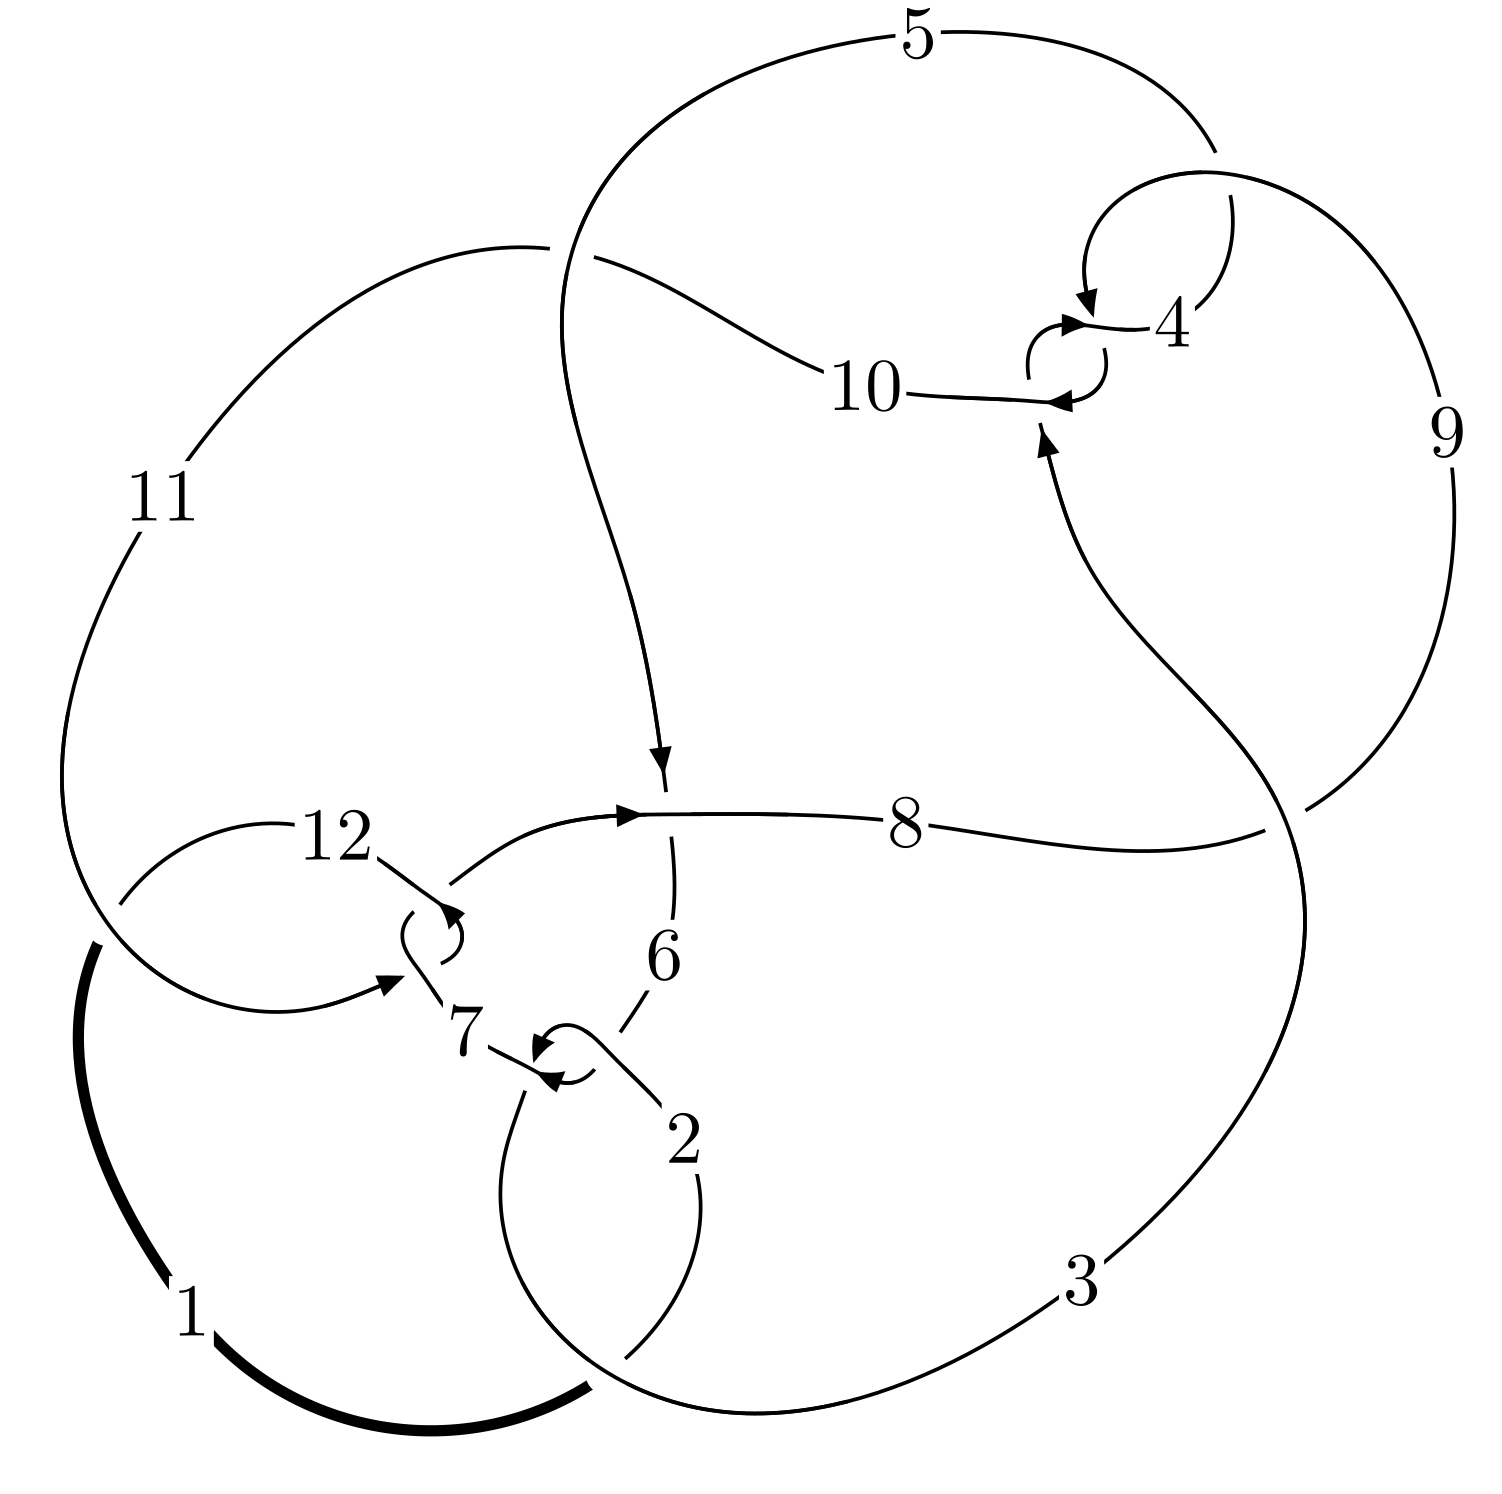
\includegraphics[width=112pt]{../../../GIT/diagram.site/Diagrams/png/2661_12n_0572.png}\\
\ \ \ A knot diagram\footnotemark}&
\allowdisplaybreaks
\textbf{Linearized knot diagam} \\
\cline{2-2}
 &
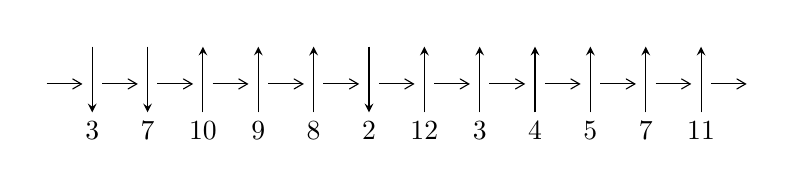
\begin{tikzpicture}[x=20pt, y=17pt]
	% nodes
	\node (C0) at (0, 0) {};
	\node (C1) at (1, 0) {};
	\node (C1U) at (1, +1) {};
	\node (C1D) at (1, -1) {3};

	\node (C2) at (2, 0) {};
	\node (C2U) at (2, +1) {};
	\node (C2D) at (2, -1) {7};

	\node (C3) at (3, 0) {};
	\node (C3U) at (3, +1) {};
	\node (C3D) at (3, -1) {10};

	\node (C4) at (4, 0) {};
	\node (C4U) at (4, +1) {};
	\node (C4D) at (4, -1) {9};

	\node (C5) at (5, 0) {};
	\node (C5U) at (5, +1) {};
	\node (C5D) at (5, -1) {8};

	\node (C6) at (6, 0) {};
	\node (C6U) at (6, +1) {};
	\node (C6D) at (6, -1) {2};

	\node (C7) at (7, 0) {};
	\node (C7U) at (7, +1) {};
	\node (C7D) at (7, -1) {12};

	\node (C8) at (8, 0) {};
	\node (C8U) at (8, +1) {};
	\node (C8D) at (8, -1) {3};

	\node (C9) at (9, 0) {};
	\node (C9U) at (9, +1) {};
	\node (C9D) at (9, -1) {4};

	\node (C10) at (10, 0) {};
	\node (C10U) at (10, +1) {};
	\node (C10D) at (10, -1) {5};

	\node (C11) at (11, 0) {};
	\node (C11U) at (11, +1) {};
	\node (C11D) at (11, -1) {7};

	\node (C12) at (12, 0) {};
	\node (C12U) at (12, +1) {};
	\node (C12D) at (12, -1) {11};
	\node (C13) at (13, 0) {};

	% arrows
	\draw[->,>={angle 60}]
	(C0) edge (C1) (C1) edge (C2) (C2) edge (C3) (C3) edge (C4) (C4) edge (C5) (C5) edge (C6) (C6) edge (C7) (C7) edge (C8) (C8) edge (C9) (C9) edge (C10) (C10) edge (C11) (C11) edge (C12) (C12) edge (C13) ;	\draw[->,>=stealth]
	(C1U) edge (C1D) (C2U) edge (C2D) (C3D) edge (C3U) (C4D) edge (C4U) (C5D) edge (C5U) (C6U) edge (C6D) (C7D) edge (C7U) (C8D) edge (C8U) (C9D) edge (C9U) (C10D) edge (C10U) (C11D) edge (C11U) (C12D) edge (C12U) ;
	\end{tikzpicture} \\
\hhline{~~} \\& 
\textbf{Solving Sequence} \\ \cline{2-2} 
 &
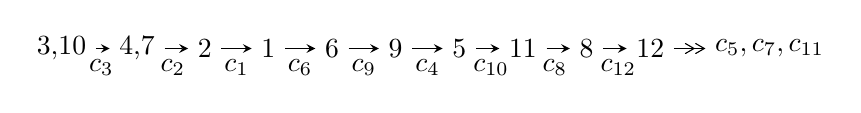
\begin{tikzpicture}[x=23pt, y=7pt]
	% node
	\node (A0) at (-1/8, 0) {3,10};
	\node (A1) at (17/16, 0) {4,7};
	\node (A2) at (17/8, 0) {2};
	\node (A3) at (25/8, 0) {1};
	\node (A4) at (33/8, 0) {6};
	\node (A5) at (41/8, 0) {9};
	\node (A6) at (49/8, 0) {5};
	\node (A7) at (57/8, 0) {11};
	\node (A8) at (65/8, 0) {8};
	\node (A9) at (73/8, 0) {12};
	\node (C1) at (1/2, -1) {$c_{3}$};
	\node (C2) at (13/8, -1) {$c_{2}$};
	\node (C3) at (21/8, -1) {$c_{1}$};
	\node (C4) at (29/8, -1) {$c_{6}$};
	\node (C5) at (37/8, -1) {$c_{9}$};
	\node (C6) at (45/8, -1) {$c_{4}$};
	\node (C7) at (53/8, -1) {$c_{10}$};
	\node (C8) at (61/8, -1) {$c_{8}$};
	\node (C9) at (69/8, -1) {$c_{12}$};
	\node (A10) at (11, 0) {$c_{5},c_{7},c_{11}$};

	% edge
	\draw[->,>=stealth]	
	(A0) edge (A1) (A1) edge (A2) (A2) edge (A3) (A3) edge (A4) (A4) edge (A5) (A5) edge (A6) (A6) edge (A7) (A7) edge (A8) (A8) edge (A9) ;
	\draw[->>,>={angle 60}]	
	(A9) edge (A10);
\end{tikzpicture} \\ 

\end{tabular} \\

\footnotetext{
The image of knot diagram is generated by the software ``\textbf{Draw programme}" developed by Andrew Bartholomew(\url{http://www.layer8.co.uk/maths/draw/index.htm\#Running-draw}), where we modified some parts for our purpose(\url{https://github.com/CATsTAILs/LinksPainter}).
}\phantom \\ \newline 
\centering \textbf{Ideals for irreducible components\footnotemark of $X_{\text{par}}$} 
 
\begin{align*}
I^u_{1}&=\langle 
2 u^{30}+2 u^{29}+\cdots+4 b+2,\;-2 u^{30}- u^{29}+\cdots+4 a-6,\;u^{31}+2 u^{30}+\cdots+2 u+2\rangle \\
I^u_{2}&=\langle 
b-1,\;2 u^3-3 u^2+3 a+3 u-3,\;u^4+3 u^2+3\rangle \\
I^u_{3}&=\langle 
- a^2 u^2+u^2 a-2 a u+b+2 a-2 u,\;-2 a^2 u^2+a^3+2 u^2 a-2 a^2-3 a u+5 a- u+1,\;u^3- u^2+2 u-1\rangle \\
I^u_{4}&=\langle 
b+1,\;- u^2+a+u-1,\;u^4+u^2-1\rangle \\
\\
I^v_{1}&=\langle 
a,\;b-1,\;v-1\rangle \\
\end{align*}
\raggedright * 5 irreducible components of $\dim_{\mathbb{C}}=0$, with total 49 representations.\\
\footnotetext{All coefficients of polynomials are rational numbers. But the coefficients are sometimes approximated in decimal forms when there is not enough margin.}
\newpage
\renewcommand{\arraystretch}{1}
\centering \section*{I. $I^u_{1}= \langle 2 u^{30}+2 u^{29}+\cdots+4 b+2,\;-2 u^{30}- u^{29}+\cdots+4 a-6,\;u^{31}+2 u^{30}+\cdots+2 u+2 \rangle$}
\flushleft \textbf{(i) Arc colorings}\\
\begin{tabular}{m{7pt} m{180pt} m{7pt} m{180pt} }
\flushright $a_{3}=$&$\begin{pmatrix}1\\0\end{pmatrix}$ \\
\flushright $a_{10}=$&$\begin{pmatrix}0\\u\end{pmatrix}$ \\
\flushright $a_{4}=$&$\begin{pmatrix}1\\- u^2\end{pmatrix}$ \\
\flushright $a_{7}=$&$\begin{pmatrix}\frac{1}{2} u^{30}+\frac{1}{4} u^{29}+\cdots+2 u+\frac{3}{2}\\-\frac{1}{2} u^{30}-\frac{1}{2} u^{29}+\cdots- u-\frac{1}{2}\end{pmatrix}$ \\
\flushright $a_{2}=$&$\begin{pmatrix}-\frac{1}{4} u^{27}-3 u^{25}+\cdots+\frac{1}{2} u+1\\\frac{1}{4} u^{27}+\frac{11}{4} u^{25}+\cdots-\frac{1}{2} u^2+\frac{1}{2} u\end{pmatrix}$ \\
\flushright $a_{1}=$&$\begin{pmatrix}-\frac{1}{4} u^{25}-\frac{5}{2} u^{23}+\cdots+u+1\\\frac{1}{4} u^{27}+\frac{11}{4} u^{25}+\cdots-\frac{1}{2} u^2+\frac{1}{2} u\end{pmatrix}$ \\
\flushright $a_{6}=$&$\begin{pmatrix}- u^{10}-5 u^8-8 u^6-3 u^4+3 u^2+1\\u^{10}+4 u^8+5 u^6-3 u^2\end{pmatrix}$ \\
\flushright $a_{9}=$&$\begin{pmatrix}- u\\u^3+u\end{pmatrix}$ \\
\flushright $a_{5}=$&$\begin{pmatrix}u^2+1\\- u^4-2 u^2\end{pmatrix}$ \\
\flushright $a_{11}=$&$\begin{pmatrix}u^5+2 u^3+u\\- u^7-3 u^5-2 u^3+u\end{pmatrix}$ \\
\flushright $a_{8}=$&$\begin{pmatrix}- u^3-2 u\\u^3+u\end{pmatrix}$ \\
\flushright $a_{12}=$&$\begin{pmatrix}\frac{1}{2} u^{30}+u^{29}+\cdots+\frac{3}{2} u+\frac{5}{2}\\-\frac{1}{4} u^{28}-\frac{1}{4} u^{27}+\cdots+\frac{3}{2} u-1\end{pmatrix}$\\&\end{tabular}
\flushleft \textbf{(ii) Obstruction class $= -1$}\\~\\
\flushleft \textbf{(iii) Cusp Shapes $= 2 u^{30}+4 u^{29}+30 u^{28}+48 u^{27}+192 u^{26}+248 u^{25}+682 u^{24}+702 u^{23}+1432 u^{22}+1112 u^{21}+1656 u^{20}+764 u^{19}+556 u^{18}-384 u^{17}-1002 u^{16}-1040 u^{15}-1088 u^{14}-344 u^{13}+216 u^{12}+568 u^{11}+830 u^{10}+454 u^9+206 u^8-108 u^7-284 u^6-180 u^5-122 u^4-6 u^3+30 u^2+4 u+12$}\\~\\
\newpage\renewcommand{\arraystretch}{1}
\flushleft \textbf{(iv) u-Polynomials at the component}\newline \\
\begin{tabular}{m{50pt}|m{274pt}}
Crossings & \hspace{64pt}u-Polynomials at each crossing \\
\hline $$\begin{aligned}c_{1}\end{aligned}$$&$\begin{aligned}
&u^{31}+44 u^{30}+\cdots+119 u+1
\end{aligned}$\\
\hline $$\begin{aligned}c_{2},c_{6}\end{aligned}$$&$\begin{aligned}
&u^{31}-2 u^{30}+\cdots+3 u-1
\end{aligned}$\\
\hline $$\begin{aligned}c_{3},c_{4},c_{9}\end{aligned}$$&$\begin{aligned}
&u^{31}+2 u^{30}+\cdots+2 u+2
\end{aligned}$\\
\hline $$\begin{aligned}c_{5}\end{aligned}$$&$\begin{aligned}
&u^{31}+7 u^{30}+\cdots-88514 u+28438
\end{aligned}$\\
\hline $$\begin{aligned}c_{7},c_{11}\end{aligned}$$&$\begin{aligned}
&u^{31}+2 u^{30}+\cdots- u-1
\end{aligned}$\\
\hline $$\begin{aligned}c_{8},c_{10}\end{aligned}$$&$\begin{aligned}
&u^{31}-2 u^{30}+\cdots-88 u+16
\end{aligned}$\\
\hline $$\begin{aligned}c_{12}\end{aligned}$$&$\begin{aligned}
&u^{31}-4 u^{30}+\cdots+39 u-1
\end{aligned}$\\
\hline
\end{tabular}\\~\\
\newpage\renewcommand{\arraystretch}{1}
\flushleft \textbf{(v) Riley Polynomials at the component}\newline \\
\begin{tabular}{m{50pt}|m{274pt}}
Crossings & \hspace{64pt}Riley Polynomials at each crossing \\
\hline $$\begin{aligned}c_{1}\end{aligned}$$&$\begin{aligned}
&y^{31}-104 y^{30}+\cdots+10991 y-1
\end{aligned}$\\
\hline $$\begin{aligned}c_{2},c_{6}\end{aligned}$$&$\begin{aligned}
&y^{31}-44 y^{30}+\cdots+119 y-1
\end{aligned}$\\
\hline $$\begin{aligned}c_{3},c_{4},c_{9}\end{aligned}$$&$\begin{aligned}
&y^{31}+26 y^{30}+\cdots+8 y-4
\end{aligned}$\\
\hline $$\begin{aligned}c_{5}\end{aligned}$$&$\begin{aligned}
&y^{31}+55 y^{30}+\cdots+4648364048 y-808719844
\end{aligned}$\\
\hline $$\begin{aligned}c_{7},c_{11}\end{aligned}$$&$\begin{aligned}
&y^{31}-4 y^{30}+\cdots+39 y-1
\end{aligned}$\\
\hline $$\begin{aligned}c_{8},c_{10}\end{aligned}$$&$\begin{aligned}
&y^{31}-14 y^{30}+\cdots+448 y-256
\end{aligned}$\\
\hline $$\begin{aligned}c_{12}\end{aligned}$$&$\begin{aligned}
&y^{31}+56 y^{30}+\cdots+479 y-1
\end{aligned}$\\
\hline
\end{tabular}\\~\\
\newpage\flushleft \textbf{(vi) Complex Volumes and Cusp Shapes}
$$\begin{array}{c|c|c}  
\text{Solutions to }I^u_{1}& \I (\text{vol} + \sqrt{-1}CS) & \text{Cusp shape}\\
 \hline 
\begin{aligned}
u &= \phantom{-}0.422005 + 0.970388 I \\
a &= \phantom{-}0.780023 - 0.122330 I \\
b &= -1.63363 - 0.20014 I\end{aligned}
 & -8.77509 - 4.02062 I & \phantom{-}3.17327 + 1.29124 I \\ \hline\begin{aligned}
u &= \phantom{-}0.422005 - 0.970388 I \\
a &= \phantom{-}0.780023 + 0.122330 I \\
b &= -1.63363 + 0.20014 I\end{aligned}
 & -8.77509 + 4.02062 I & \phantom{-}3.17327 - 1.29124 I \\ \hline\begin{aligned}
u &= -0.438452 + 0.819465 I \\
a &= \phantom{-}0.612911 + 0.875111 I \\
b &= -1.66514 - 0.05832 I\end{aligned}
 & -9.30026 - 3.06037 I & \phantom{-}2.53545 + 3.57264 I \\ \hline\begin{aligned}
u &= -0.438452 - 0.819465 I \\
a &= \phantom{-}0.612911 - 0.875111 I \\
b &= -1.66514 + 0.05832 I\end{aligned}
 & -9.30026 + 3.06037 I & \phantom{-}2.53545 - 3.57264 I \\ \hline\begin{aligned}
u &= -0.151148 + 1.120390 I \\
a &= -0.774438 + 0.936580 I \\
b &= \phantom{-}0.430006 - 0.577254 I\end{aligned}
 & -1.40117 + 1.17674 I & \phantom{-}6.48562 - 3.33148 I \\ \hline\begin{aligned}
u &= -0.151148 - 1.120390 I \\
a &= -0.774438 - 0.936580 I \\
b &= \phantom{-}0.430006 + 0.577254 I\end{aligned}
 & -1.40117 - 1.17674 I & \phantom{-}6.48562 + 3.33148 I \\ \hline\begin{aligned}
u &= \phantom{-}0.822269 + 0.212623 I \\
a &= -1.60479 + 1.78111 I \\
b &= \phantom{-}1.64313 - 0.27195 I\end{aligned}
 & -6.42043 + 8.50954 I & \phantom{-}6.05681 - 5.42341 I \\ \hline\begin{aligned}
u &= \phantom{-}0.822269 - 0.212623 I \\
a &= -1.60479 - 1.78111 I \\
b &= \phantom{-}1.64313 + 0.27195 I\end{aligned}
 & -6.42043 - 8.50954 I & \phantom{-}6.05681 + 5.42341 I \\ \hline\begin{aligned}
u &= -0.769464 + 0.275211 I \\
a &= -1.58833 - 1.20476 I \\
b &= \phantom{-}1.68783 + 0.04109 I\end{aligned}
 & -7.55262 - 1.26507 I & \phantom{-}4.68154 + 1.47900 I \\ \hline\begin{aligned}
u &= -0.769464 - 0.275211 I \\
a &= -1.58833 + 1.20476 I \\
b &= \phantom{-}1.68783 - 0.04109 I\end{aligned}
 & -7.55262 + 1.26507 I & \phantom{-}4.68154 - 1.47900 I\\
 \hline 
 \end{array}$$\newpage$$\begin{array}{c|c|c}  
\text{Solutions to }I^u_{1}& \I (\text{vol} + \sqrt{-1}CS) & \text{Cusp shape}\\
 \hline 
\begin{aligned}
u &= \phantom{-}0.801134\phantom{ +0.000000I} \\
a &= \phantom{-}1.76838\phantom{ +0.000000I} \\
b &= -1.08175\phantom{ +0.000000I}\end{aligned}
 & \phantom{-}2.34779\phantom{ +0.000000I} & \phantom{-}4.38740\phantom{ +0.000000I} \\ \hline\begin{aligned}
u &= -0.777905\phantom{ +0.000000I} \\
a &= -0.722824\phantom{ +0.000000I} \\
b &= -0.0906547\phantom{ +0.000000I}\end{aligned}
 & \phantom{-}5.57117\phantom{ +0.000000I} & \phantom{-}16.4750\phantom{ +0.000000I} \\ \hline\begin{aligned}
u &= -0.709050 + 0.173396 I \\
a &= \phantom{-}0.38023 + 2.22913 I \\
b &= -0.614830 - 0.764424 I\end{aligned}
 & \phantom{-}1.18939 - 4.50976 I & \phantom{-}8.37255 + 6.79420 I \\ \hline\begin{aligned}
u &= -0.709050 - 0.173396 I \\
a &= \phantom{-}0.38023 - 2.22913 I \\
b &= -0.614830 + 0.764424 I\end{aligned}
 & \phantom{-}1.18939 + 4.50976 I & \phantom{-}8.37255 - 6.79420 I \\ \hline\begin{aligned}
u &= -0.332218 + 1.265660 I \\
a &= \phantom{-}0.704768 + 0.124425 I \\
b &= \phantom{-}0.095778 - 0.113924 I\end{aligned}
 & \phantom{-}1.64712 - 4.00353 I & \phantom{-}11.89002 + 3.58978 I \\ \hline\begin{aligned}
u &= -0.332218 - 1.265660 I \\
a &= \phantom{-}0.704768 - 0.124425 I \\
b &= \phantom{-}0.095778 + 0.113924 I\end{aligned}
 & \phantom{-}1.64712 + 4.00353 I & \phantom{-}11.89002 - 3.58978 I \\ \hline\begin{aligned}
u &= \phantom{-}0.355714 + 1.276500 I \\
a &= -0.665256 + 0.850651 I \\
b &= \phantom{-}1.105160 + 0.056084 I\end{aligned}
 & -1.62439 + 4.16232 I & \phantom{-}0.18076 - 3.51312 I \\ \hline\begin{aligned}
u &= \phantom{-}0.355714 - 1.276500 I \\
a &= -0.665256 - 0.850651 I \\
b &= \phantom{-}1.105160 - 0.056084 I\end{aligned}
 & -1.62439 - 4.16232 I & \phantom{-}0.18076 + 3.51312 I \\ \hline\begin{aligned}
u &= -0.054498 + 1.374780 I \\
a &= -0.492915 - 0.029751 I \\
b &= -0.992043 + 0.551725 I\end{aligned}
 & -6.79962 + 0.91660 I & -1.89239 - 1.83526 I \\ \hline\begin{aligned}
u &= -0.054498 - 1.374780 I \\
a &= -0.492915 + 0.029751 I \\
b &= -0.992043 - 0.551725 I\end{aligned}
 & -6.79962 - 0.91660 I & -1.89239 + 1.83526 I\\
 \hline 
 \end{array}$$\newpage$$\begin{array}{c|c|c}  
\text{Solutions to }I^u_{1}& \I (\text{vol} + \sqrt{-1}CS) & \text{Cusp shape}\\
 \hline 
\begin{aligned}
u &= -0.292248 + 1.364020 I \\
a &= \phantom{-}0.75119 - 1.48738 I \\
b &= \phantom{-}0.689770 + 0.858986 I\end{aligned}
 & -3.67517 - 8.15180 I & \phantom{-}3.05070 + 7.43504 I \\ \hline\begin{aligned}
u &= -0.292248 - 1.364020 I \\
a &= \phantom{-}0.75119 + 1.48738 I \\
b &= \phantom{-}0.689770 - 0.858986 I\end{aligned}
 & -3.67517 + 8.15180 I & \phantom{-}3.05070 - 7.43504 I \\ \hline\begin{aligned}
u &= \phantom{-}0.34385 + 1.39505 I \\
a &= -0.22148 - 2.07364 I \\
b &= -1.66852 + 0.31356 I\end{aligned}
 & -11.5166 + 12.7194 I & \phantom{-}2.07160 - 6.66192 I \\ \hline\begin{aligned}
u &= \phantom{-}0.34385 - 1.39505 I \\
a &= -0.22148 + 2.07364 I \\
b &= -1.66852 - 0.31356 I\end{aligned}
 & -11.5166 - 12.7194 I & \phantom{-}2.07160 + 6.66192 I \\ \hline\begin{aligned}
u &= -0.30540 + 1.41307 I \\
a &= -0.24753 + 1.59262 I \\
b &= -1.74843 - 0.08810 I\end{aligned}
 & -12.92960 - 5.15155 I & \phantom{-}0.52455 + 2.55322 I \\ \hline\begin{aligned}
u &= -0.30540 - 1.41307 I \\
a &= -0.24753 - 1.59262 I \\
b &= -1.74843 + 0.08810 I\end{aligned}
 & -12.92960 + 5.15155 I & \phantom{-}0.52455 - 2.55322 I \\ \hline\begin{aligned}
u &= -0.047932 + 0.529217 I \\
a &= -0.316164 + 0.652908 I \\
b &= \phantom{-}0.693120 - 0.435687 I\end{aligned}
 & -1.07809 + 1.45065 I & \phantom{-}1.68946 - 3.85910 I \\ \hline\begin{aligned}
u &= -0.047932 - 0.529217 I \\
a &= -0.316164 - 0.652908 I \\
b &= \phantom{-}0.693120 + 0.435687 I\end{aligned}
 & -1.07809 - 1.45065 I & \phantom{-}1.68946 + 3.85910 I \\ \hline\begin{aligned}
u &= -0.02824 + 1.47075 I \\
a &= \phantom{-}1.096690 - 0.319605 I \\
b &= \phantom{-}1.77899 + 0.14272 I\end{aligned}
 & -16.7493 - 3.9918 I & -1.06457 + 2.30903 I \\ \hline\begin{aligned}
u &= -0.02824 - 1.47075 I \\
a &= \phantom{-}1.096690 + 0.319605 I \\
b &= \phantom{-}1.77899 - 0.14272 I\end{aligned}
 & -16.7493 + 3.9918 I & -1.06457 - 2.30903 I\\
 \hline 
 \end{array}$$\newpage$$\begin{array}{c|c|c}  
\text{Solutions to }I^u_{1}& \I (\text{vol} + \sqrt{-1}CS) & \text{Cusp shape}\\
 \hline 
\begin{aligned}
u &= \phantom{-}0.346395\phantom{ +0.000000I} \\
a &= \phantom{-}2.12463\phantom{ +0.000000I} \\
b &= -0.429962\phantom{ +0.000000I}\end{aligned}
 & \phantom{-}0.849256\phantom{ +0.000000I} & \phantom{-}13.6270\phantom{ +0.000000I}\\
 \hline 
 \end{array}$$\newpage\newpage\renewcommand{\arraystretch}{1}
\centering \section*{II. $I^u_{2}= \langle b-1,\;2 u^3-3 u^2+3 a+3 u-3,\;u^4+3 u^2+3 \rangle$}
\flushleft \textbf{(i) Arc colorings}\\
\begin{tabular}{m{7pt} m{180pt} m{7pt} m{180pt} }
\flushright $a_{3}=$&$\begin{pmatrix}1\\0\end{pmatrix}$ \\
\flushright $a_{10}=$&$\begin{pmatrix}0\\u\end{pmatrix}$ \\
\flushright $a_{4}=$&$\begin{pmatrix}1\\- u^2\end{pmatrix}$ \\
\flushright $a_{7}=$&$\begin{pmatrix}-\frac{2}{3} u^3+u^2- u+1\\1\end{pmatrix}$ \\
\flushright $a_{2}=$&$\begin{pmatrix}\frac{2}{3} u^3- u^2+u\\-1\end{pmatrix}$ \\
\flushright $a_{1}=$&$\begin{pmatrix}\frac{2}{3} u^3- u^2+u-1\\-1\end{pmatrix}$ \\
\flushright $a_{6}=$&$\begin{pmatrix}1\\0\end{pmatrix}$ \\
\flushright $a_{9}=$&$\begin{pmatrix}- u\\u^3+u\end{pmatrix}$ \\
\flushright $a_{5}=$&$\begin{pmatrix}u^2+1\\u^2+3\end{pmatrix}$ \\
\flushright $a_{11}=$&$\begin{pmatrix}- u^3-2 u\\u^3+u\end{pmatrix}$ \\
\flushright $a_{8}=$&$\begin{pmatrix}- u^3-2 u\\u^3+u\end{pmatrix}$ \\
\flushright $a_{12}=$&$\begin{pmatrix}-\frac{1}{3} u^3- u^2- u-1\\u^3+u-1\end{pmatrix}$\\&\end{tabular}
\flushleft \textbf{(ii) Obstruction class $= 1$}\\~\\
\flushleft \textbf{(iii) Cusp Shapes $= -4 u^2$}\\~\\
\newpage\renewcommand{\arraystretch}{1}
\flushleft \textbf{(iv) u-Polynomials at the component}\newline \\
\begin{tabular}{m{50pt}|m{274pt}}
Crossings & \hspace{64pt}u-Polynomials at each crossing \\
\hline $$\begin{aligned}c_{1},c_{2},c_{11}\\c_{12}\end{aligned}$$&$\begin{aligned}
&(u-1)^4
\end{aligned}$\\
\hline $$\begin{aligned}c_{3},c_{4},c_{9}\end{aligned}$$&$\begin{aligned}
&u^4+3 u^2+3
\end{aligned}$\\
\hline $$\begin{aligned}c_{5},c_{8},c_{10}\end{aligned}$$&$\begin{aligned}
&u^4-3 u^2+3
\end{aligned}$\\
\hline $$\begin{aligned}c_{6},c_{7}\end{aligned}$$&$\begin{aligned}
&(u+1)^4
\end{aligned}$\\
\hline
\end{tabular}\\~\\
\newpage\renewcommand{\arraystretch}{1}
\flushleft \textbf{(v) Riley Polynomials at the component}\newline \\
\begin{tabular}{m{50pt}|m{274pt}}
Crossings & \hspace{64pt}Riley Polynomials at each crossing \\
\hline $$\begin{aligned}c_{1},c_{2},c_{6}\\c_{7},c_{11},c_{12}\end{aligned}$$&$\begin{aligned}
&(y-1)^4
\end{aligned}$\\
\hline $$\begin{aligned}c_{3},c_{4},c_{9}\end{aligned}$$&$\begin{aligned}
&(y^2+3 y+3)^2
\end{aligned}$\\
\hline $$\begin{aligned}c_{5},c_{8},c_{10}\end{aligned}$$&$\begin{aligned}
&(y^2-3 y+3)^2
\end{aligned}$\\
\hline
\end{tabular}\\~\\
\newpage\flushleft \textbf{(vi) Complex Volumes and Cusp Shapes}
$$\begin{array}{c|c|c}  
\text{Solutions to }I^u_{2}& \I (\text{vol} + \sqrt{-1}CS) & \text{Cusp shape}\\
 \hline 
\begin{aligned}
u &= \phantom{-}0.340625 + 1.271230 I \\
a &= \phantom{-}0.233945 + 0.669365 I \\
b &= \phantom{-}1.00000\phantom{ +0.000000I}\end{aligned}
 & \phantom{-0.000000 -}4.05977 I & \phantom{-}6.00000 - 3.46410 I \\ \hline\begin{aligned}
u &= \phantom{-}0.340625 - 1.271230 I \\
a &= \phantom{-}0.233945 - 0.669365 I \\
b &= \phantom{-}1.00000\phantom{ +0.000000I}\end{aligned}
 & \phantom{-0.000000 } -4.05977 I & \phantom{-}6.00000 + 3.46410 I \\ \hline\begin{aligned}
u &= -0.340625 + 1.271230 I \\
a &= -1.23394 - 1.06269 I \\
b &= \phantom{-}1.00000\phantom{ +0.000000I}\end{aligned}
 & \phantom{-0.000000 } -4.05977 I & \phantom{-}6.00000 + 3.46410 I \\ \hline\begin{aligned}
u &= -0.340625 - 1.271230 I \\
a &= -1.23394 + 1.06269 I \\
b &= \phantom{-}1.00000\phantom{ +0.000000I}\end{aligned}
 & \phantom{-0.000000 -}4.05977 I & \phantom{-}6.00000 - 3.46410 I\\
 \hline 
 \end{array}$$\newpage\newpage\renewcommand{\arraystretch}{1}
\centering \section*{III. $I^u_{3}= \langle - a^2 u^2+u^2 a-2 a u+b+2 a-2 u,\;-2 a^2 u^2+2 u^2 a+\cdots+5 a+1,\;u^3- u^2+2 u-1 \rangle$}
\flushleft \textbf{(i) Arc colorings}\\
\begin{tabular}{m{7pt} m{180pt} m{7pt} m{180pt} }
\flushright $a_{3}=$&$\begin{pmatrix}1\\0\end{pmatrix}$ \\
\flushright $a_{10}=$&$\begin{pmatrix}0\\u\end{pmatrix}$ \\
\flushright $a_{4}=$&$\begin{pmatrix}1\\- u^2\end{pmatrix}$ \\
\flushright $a_{7}=$&$\begin{pmatrix}a\\a^2 u^2- u^2 a+2 a u-2 a+2 u\end{pmatrix}$ \\
\flushright $a_{2}=$&$\begin{pmatrix}a^2 u^2+2 a u- a+2 u\\a^2 u- u^2 a- a^2+2 a u-2 u^2+2 u-2\end{pmatrix}$ \\
\flushright $a_{1}=$&$\begin{pmatrix}a^2 u^2+a^2 u- u^2 a- a^2+4 a u-2 u^2- a+4 u-2\\a^2 u- u^2 a- a^2+2 a u-2 u^2+2 u-2\end{pmatrix}$ \\
\flushright $a_{6}=$&$\begin{pmatrix}u^2+1\\- u^2+u-1\end{pmatrix}$ \\
\flushright $a_{9}=$&$\begin{pmatrix}- u\\u^2- u+1\end{pmatrix}$ \\
\flushright $a_{5}=$&$\begin{pmatrix}u^2+1\\- u^2+u-1\end{pmatrix}$ \\
\flushright $a_{11}=$&$\begin{pmatrix}1\\0\end{pmatrix}$ \\
\flushright $a_{8}=$&$\begin{pmatrix}- u^2-1\\u^2- u+1\end{pmatrix}$ \\
\flushright $a_{12}=$&$\begin{pmatrix}a^2 u^2+2 a u- a+2 u\\a^2 u- u^2 a- a^2+2 a u-2 u^2+2 u-2\end{pmatrix}$\\&\end{tabular}
\flushleft \textbf{(ii) Obstruction class $= -1$}\\~\\
\flushleft \textbf{(iii) Cusp Shapes $= 4 u^2-4 u+10$}\\~\\
\newpage\renewcommand{\arraystretch}{1}
\flushleft \textbf{(iv) u-Polynomials at the component}\newline \\
\begin{tabular}{m{50pt}|m{274pt}}
Crossings & \hspace{64pt}u-Polynomials at each crossing \\
\hline $$\begin{aligned}c_{1}\end{aligned}$$&$\begin{aligned}
&u^9+6 u^8+15 u^7+21 u^6+19 u^5+12 u^4+7 u^3+5 u^2+2 u+1
\end{aligned}$\\
\hline $$\begin{aligned}c_{2},c_{6},c_{7}\\c_{11}\end{aligned}$$&$\begin{aligned}
&u^9-3 u^7- u^6+3 u^5+2 u^4- u^3- u^2+1
\end{aligned}$\\
\hline $$\begin{aligned}c_{3},c_{4},c_{9}\end{aligned}$$&$\begin{aligned}
&(u^3- u^2+2 u-1)^3
\end{aligned}$\\
\hline $$\begin{aligned}c_{5}\end{aligned}$$&$\begin{aligned}
&u^9
\end{aligned}$\\
\hline $$\begin{aligned}c_{8},c_{10}\end{aligned}$$&$\begin{aligned}
&(u^3+u^2-1)^3
\end{aligned}$\\
\hline $$\begin{aligned}c_{12}\end{aligned}$$&$\begin{aligned}
&u^9-6 u^8+15 u^7-21 u^6+19 u^5-12 u^4+7 u^3-5 u^2+2 u-1
\end{aligned}$\\
\hline
\end{tabular}\\~\\
\newpage\renewcommand{\arraystretch}{1}
\flushleft \textbf{(v) Riley Polynomials at the component}\newline \\
\begin{tabular}{m{50pt}|m{274pt}}
Crossings & \hspace{64pt}Riley Polynomials at each crossing \\
\hline $$\begin{aligned}c_{1},c_{12}\end{aligned}$$&$\begin{aligned}
&y^9-6 y^8+11 y^7- y^6+11 y^5-40 y^4-37 y^3-21 y^2-6 y-1
\end{aligned}$\\
\hline $$\begin{aligned}c_{2},c_{6},c_{7}\\c_{11}\end{aligned}$$&$\begin{aligned}
&y^9-6 y^8+15 y^7-21 y^6+19 y^5-12 y^4+7 y^3-5 y^2+2 y-1
\end{aligned}$\\
\hline $$\begin{aligned}c_{3},c_{4},c_{9}\end{aligned}$$&$\begin{aligned}
&(y^3+3 y^2+2 y-1)^3
\end{aligned}$\\
\hline $$\begin{aligned}c_{5}\end{aligned}$$&$\begin{aligned}
&y^9
\end{aligned}$\\
\hline $$\begin{aligned}c_{8},c_{10}\end{aligned}$$&$\begin{aligned}
&(y^3- y^2+2 y-1)^3
\end{aligned}$\\
\hline
\end{tabular}\\~\\
\newpage\flushleft \textbf{(vi) Complex Volumes and Cusp Shapes}
$$\begin{array}{c|c|c}  
\text{Solutions to }I^u_{3}& \I (\text{vol} + \sqrt{-1}CS) & \text{Cusp shape}\\
 \hline 
\begin{aligned}
u &= \phantom{-}0.215080 + 1.307140 I \\
a &= -1.110710 - 0.304480 I \\
b &= -1.324820 - 0.175904 I\end{aligned}
 & -3.02413 + 2.82812 I & \phantom{-}2.49024 - 2.97945 I \\ \hline\begin{aligned}
u &= \phantom{-}0.215080 + 1.307140 I \\
a &= -0.633796 - 0.350292 I \\
b &= \phantom{-}0.376870 + 0.700062 I\end{aligned}
 & -3.02413 + 2.82812 I & \phantom{-}2.49024 - 2.97945 I \\ \hline\begin{aligned}
u &= \phantom{-}0.215080 + 1.307140 I \\
a &= \phantom{-}0.41979 + 1.77933 I \\
b &= \phantom{-}0.947946 - 0.524157 I\end{aligned}
 & -3.02413 + 2.82812 I & \phantom{-}2.49024 - 2.97945 I \\ \hline\begin{aligned}
u &= \phantom{-}0.215080 - 1.307140 I \\
a &= -1.110710 + 0.304480 I \\
b &= -1.324820 + 0.175904 I\end{aligned}
 & -3.02413 - 2.82812 I & \phantom{-}2.49024 + 2.97945 I \\ \hline\begin{aligned}
u &= \phantom{-}0.215080 - 1.307140 I \\
a &= -0.633796 + 0.350292 I \\
b &= \phantom{-}0.376870 - 0.700062 I\end{aligned}
 & -3.02413 - 2.82812 I & \phantom{-}2.49024 + 2.97945 I \\ \hline\begin{aligned}
u &= \phantom{-}0.215080 - 1.307140 I \\
a &= \phantom{-}0.41979 - 1.77933 I \\
b &= \phantom{-}0.947946 + 0.524157 I\end{aligned}
 & -3.02413 - 2.82812 I & \phantom{-}2.49024 + 2.97945 I \\ \hline\begin{aligned}
u &= \phantom{-}0.569840\phantom{ +0.000000I} \\
a &= -0.101925\phantom{ +0.000000I} \\
b &= \phantom{-}1.26384\phantom{ +0.000000I}\end{aligned}
 & \phantom{-}1.11345\phantom{ +0.000000I} & \phantom{-}9.01950\phantom{ +0.000000I} \\ \hline\begin{aligned}
u &= \phantom{-}0.569840\phantom{ +0.000000I} \\
a &= \phantom{-}1.37568 + 1.52573 I \\
b &= -0.631920 - 0.444935 I\end{aligned}
 & \phantom{-}1.11345\phantom{ +0.000000I} & \phantom{-}9.01950\phantom{ +0.000000I} \\ \hline\begin{aligned}
u &= \phantom{-}0.569840\phantom{ +0.000000I} \\
a &= \phantom{-}1.37568 - 1.52573 I \\
b &= -0.631920 + 0.444935 I\end{aligned}
 & \phantom{-}1.11345\phantom{ +0.000000I} & \phantom{-}9.01950\phantom{ +0.000000I}\\
 \hline 
 \end{array}$$\newpage\newpage\renewcommand{\arraystretch}{1}
\centering \section*{IV. $I^u_{4}= \langle b+1,\;- u^2+a+u-1,\;u^4+u^2-1 \rangle$}
\flushleft \textbf{(i) Arc colorings}\\
\begin{tabular}{m{7pt} m{180pt} m{7pt} m{180pt} }
\flushright $a_{3}=$&$\begin{pmatrix}1\\0\end{pmatrix}$ \\
\flushright $a_{10}=$&$\begin{pmatrix}0\\u\end{pmatrix}$ \\
\flushright $a_{4}=$&$\begin{pmatrix}1\\- u^2\end{pmatrix}$ \\
\flushright $a_{7}=$&$\begin{pmatrix}u^2- u+1\\-1\end{pmatrix}$ \\
\flushright $a_{2}=$&$\begin{pmatrix}u^2- u+2\\-1\end{pmatrix}$ \\
\flushright $a_{1}=$&$\begin{pmatrix}u^2- u+1\\-1\end{pmatrix}$ \\
\flushright $a_{6}=$&$\begin{pmatrix}-1\\0\end{pmatrix}$ \\
\flushright $a_{9}=$&$\begin{pmatrix}- u\\u^3+u\end{pmatrix}$ \\
\flushright $a_{5}=$&$\begin{pmatrix}u^2+1\\- u^2-1\end{pmatrix}$ \\
\flushright $a_{11}=$&$\begin{pmatrix}u^3+2 u\\- u^3- u\end{pmatrix}$ \\
\flushright $a_{8}=$&$\begin{pmatrix}- u^3-2 u\\u^3+u\end{pmatrix}$ \\
\flushright $a_{12}=$&$\begin{pmatrix}u^3+u^2+u+1\\- u^3- u-1\end{pmatrix}$\\&\end{tabular}
\flushleft \textbf{(ii) Obstruction class $= 1$}\\~\\
\flushleft \textbf{(iii) Cusp Shapes $= 4 u^2+8$}\\~\\
\newpage\renewcommand{\arraystretch}{1}
\flushleft \textbf{(iv) u-Polynomials at the component}\newline \\
\begin{tabular}{m{50pt}|m{274pt}}
Crossings & \hspace{64pt}u-Polynomials at each crossing \\
\hline $$\begin{aligned}c_{1},c_{6},c_{7}\\c_{12}\end{aligned}$$&$\begin{aligned}
&(u-1)^4
\end{aligned}$\\
\hline $$\begin{aligned}c_{2},c_{11}\end{aligned}$$&$\begin{aligned}
&(u+1)^4
\end{aligned}$\\
\hline $$\begin{aligned}c_{3},c_{4},c_{9}\end{aligned}$$&$\begin{aligned}
&u^4+u^2-1
\end{aligned}$\\
\hline $$\begin{aligned}c_{5},c_{8},c_{10}\end{aligned}$$&$\begin{aligned}
&u^4- u^2-1
\end{aligned}$\\
\hline
\end{tabular}\\~\\
\newpage\renewcommand{\arraystretch}{1}
\flushleft \textbf{(v) Riley Polynomials at the component}\newline \\
\begin{tabular}{m{50pt}|m{274pt}}
Crossings & \hspace{64pt}Riley Polynomials at each crossing \\
\hline $$\begin{aligned}c_{1},c_{2},c_{6}\\c_{7},c_{11},c_{12}\end{aligned}$$&$\begin{aligned}
&(y-1)^4
\end{aligned}$\\
\hline $$\begin{aligned}c_{3},c_{4},c_{9}\end{aligned}$$&$\begin{aligned}
&(y^2+y-1)^2
\end{aligned}$\\
\hline $$\begin{aligned}c_{5},c_{8},c_{10}\end{aligned}$$&$\begin{aligned}
&(y^2- y-1)^2
\end{aligned}$\\
\hline
\end{tabular}\\~\\
\newpage\flushleft \textbf{(vi) Complex Volumes and Cusp Shapes}
$$\begin{array}{c|c|c}  
\text{Solutions to }I^u_{4}& \I (\text{vol} + \sqrt{-1}CS) & \text{Cusp shape}\\
 \hline 
\begin{aligned}
u &= \phantom{-}0.786151\phantom{ +0.000000I} \\
a &= \phantom{-}0.831883\phantom{ +0.000000I} \\
b &= -1.00000\phantom{ +0.000000I}\end{aligned}
 & \phantom{-}3.94784\phantom{ +0.000000I} & \phantom{-}10.4720\phantom{ +0.000000I} \\ \hline\begin{aligned}
u &= -0.786151\phantom{ +0.000000I} \\
a &= \phantom{-}2.40419\phantom{ +0.000000I} \\
b &= -1.00000\phantom{ +0.000000I}\end{aligned}
 & \phantom{-}3.94784\phantom{ +0.000000I} & \phantom{-}10.4720\phantom{ +0.000000I} \\ \hline\begin{aligned}
u &= \phantom{-0.000000 -}1.272020 I \\
a &= -0.618030 - 1.272020 I \\
b &= -1.00000\phantom{ +0.000000I}\end{aligned}
 & -3.94784\phantom{ +0.000000I} & \phantom{-}1.52790\phantom{ +0.000000I} \\ \hline\begin{aligned}
u &= \phantom{-0.000000 } -1.272020 I \\
a &= -0.618030 + 1.272020 I \\
b &= -1.00000\phantom{ +0.000000I}\end{aligned}
 & -3.94784\phantom{ +0.000000I} & \phantom{-}1.52790\phantom{ +0.000000I}\\
 \hline 
 \end{array}$$\newpage\newpage\renewcommand{\arraystretch}{1}
\centering \section*{V. $I^v_{1}= \langle a,\;b-1,\;v-1 \rangle$}
\flushleft \textbf{(i) Arc colorings}\\
\begin{tabular}{m{7pt} m{180pt} m{7pt} m{180pt} }
\flushright $a_{3}=$&$\begin{pmatrix}1\\0\end{pmatrix}$ \\
\flushright $a_{10}=$&$\begin{pmatrix}1\\0\end{pmatrix}$ \\
\flushright $a_{4}=$&$\begin{pmatrix}1\\0\end{pmatrix}$ \\
\flushright $a_{7}=$&$\begin{pmatrix}0\\1\end{pmatrix}$ \\
\flushright $a_{2}=$&$\begin{pmatrix}1\\-1\end{pmatrix}$ \\
\flushright $a_{1}=$&$\begin{pmatrix}0\\-1\end{pmatrix}$ \\
\flushright $a_{6}=$&$\begin{pmatrix}1\\0\end{pmatrix}$ \\
\flushright $a_{9}=$&$\begin{pmatrix}1\\0\end{pmatrix}$ \\
\flushright $a_{5}=$&$\begin{pmatrix}1\\0\end{pmatrix}$ \\
\flushright $a_{11}=$&$\begin{pmatrix}1\\0\end{pmatrix}$ \\
\flushright $a_{8}=$&$\begin{pmatrix}1\\0\end{pmatrix}$ \\
\flushright $a_{12}=$&$\begin{pmatrix}1\\-1\end{pmatrix}$\\&\end{tabular}
\flushleft \textbf{(ii) Obstruction class $= 1$}\\~\\
\flushleft \textbf{(iii) Cusp Shapes $= 0$}\\~\\
\newpage\renewcommand{\arraystretch}{1}
\flushleft \textbf{(iv) u-Polynomials at the component}\newline \\
\begin{tabular}{m{50pt}|m{274pt}}
Crossings & \hspace{64pt}u-Polynomials at each crossing \\
\hline $$\begin{aligned}c_{1},c_{2},c_{11}\\c_{12}\end{aligned}$$&$\begin{aligned}
&u-1
\end{aligned}$\\
\hline $$\begin{aligned}c_{3},c_{4},c_{5}\\c_{8},c_{9},c_{10}\end{aligned}$$&$\begin{aligned}
&u
\end{aligned}$\\
\hline $$\begin{aligned}c_{6},c_{7}\end{aligned}$$&$\begin{aligned}
&u+1
\end{aligned}$\\
\hline
\end{tabular}\\~\\
\newpage\renewcommand{\arraystretch}{1}
\flushleft \textbf{(v) Riley Polynomials at the component}\newline \\
\begin{tabular}{m{50pt}|m{274pt}}
Crossings & \hspace{64pt}Riley Polynomials at each crossing \\
\hline $$\begin{aligned}c_{1},c_{2},c_{6}\\c_{7},c_{11},c_{12}\end{aligned}$$&$\begin{aligned}
&y-1
\end{aligned}$\\
\hline $$\begin{aligned}c_{3},c_{4},c_{5}\\c_{8},c_{9},c_{10}\end{aligned}$$&$\begin{aligned}
&y
\end{aligned}$\\
\hline
\end{tabular}\\~\\
\newpage\flushleft \textbf{(vi) Complex Volumes and Cusp Shapes}
$$\begin{array}{c|c|c}  
\text{Solutions to }I^v_{1}& \I (\text{vol} + \sqrt{-1}CS) & \text{Cusp shape}\\
 \hline 
\begin{aligned}
v &= \phantom{-}1.00000\phantom{ +0.000000I} \\
a &= \phantom{-0.000000 } 0 \\
b &= \phantom{-}1.00000\phantom{ +0.000000I}\end{aligned}
 & \phantom{-0.000000 } 0 & \phantom{-0.000000 } 0\\
 \hline 
 \end{array}$$\newpage
\newpage\renewcommand{\arraystretch}{1}
\centering \section*{ VI. u-Polynomials}
\begin{tabular}{m{50pt}|m{274pt}}
Crossings & \hspace{64pt}u-Polynomials at each crossing \\
\hline $$\begin{aligned}c_{1}\end{aligned}$$&$\begin{aligned}
&((u-1)^9)(u^9+6 u^8+\cdots+2 u+1)\\
&\cdot(u^{31}+44 u^{30}+\cdots+119 u+1)
\end{aligned}$\\
\hline $$\begin{aligned}c_{2}\end{aligned}$$&$\begin{aligned}
&(u-1)^5(u+1)^4(u^9-3 u^7- u^6+3 u^5+2 u^4- u^3- u^2+1)\\
&\cdot(u^{31}-2 u^{30}+\cdots+3 u-1)
\end{aligned}$\\
\hline $$\begin{aligned}c_{3},c_{4},c_{9}\end{aligned}$$&$\begin{aligned}
&u(u^{3}-u^{2}+2 u-1)^{3}(u^4+u^2-1)(u^4+3 u^2+3)(u^{31}+2 u^{30}+\cdots+2 u+2)
\end{aligned}$\\
\hline $$\begin{aligned}c_{5}\end{aligned}$$&$\begin{aligned}
&u^{10}(u^4-3 u^2+3)(u^4- u^2-1)(u^{31}+7 u^{30}+\cdots-88514 u+28438)
\end{aligned}$\\
\hline $$\begin{aligned}c_{6}\end{aligned}$$&$\begin{aligned}
&(u-1)^4(u+1)^5(u^9-3 u^7- u^6+3 u^5+2 u^4- u^3- u^2+1)\\
&\cdot(u^{31}-2 u^{30}+\cdots+3 u-1)
\end{aligned}$\\
\hline $$\begin{aligned}c_{7}\end{aligned}$$&$\begin{aligned}
&(u-1)^4(u+1)^5(u^9-3 u^7- u^6+3 u^5+2 u^4- u^3- u^2+1)\\
&\cdot(u^{31}+2 u^{30}+\cdots- u-1)
\end{aligned}$\\
\hline $$\begin{aligned}c_{8},c_{10}\end{aligned}$$&$\begin{aligned}
&u(u^3+u^2-1)^{3}(u^4-3 u^2+3)(u^4- u^2-1)(u^{31}-2 u^{30}+\cdots-88 u+16)
\end{aligned}$\\
\hline $$\begin{aligned}c_{11}\end{aligned}$$&$\begin{aligned}
&(u-1)^5(u+1)^4(u^9-3 u^7- u^6+3 u^5+2 u^4- u^3- u^2+1)\\
&\cdot(u^{31}+2 u^{30}+\cdots- u-1)
\end{aligned}$\\
\hline $$\begin{aligned}c_{12}\end{aligned}$$&$\begin{aligned}
&((u-1)^9)(u^9-6 u^8+\cdots+2 u-1)\\
&\cdot(u^{31}-4 u^{30}+\cdots+39 u-1)
\end{aligned}$\\
\hline
\end{tabular}\newpage\renewcommand{\arraystretch}{1}
\centering \section*{ VII. Riley Polynomials}
\begin{tabular}{m{50pt}|m{274pt}}
Crossings & \hspace{64pt}Riley Polynomials at each crossing \\
\hline $$\begin{aligned}c_{1}\end{aligned}$$&$\begin{aligned}
&((y-1)^9)(y^9-6 y^8+\cdots-6 y-1)\\
&\cdot(y^{31}-104 y^{30}+\cdots+10991 y-1)
\end{aligned}$\\
\hline $$\begin{aligned}c_{2},c_{6}\end{aligned}$$&$\begin{aligned}
&((y-1)^9)(y^9-6 y^8+\cdots+2 y-1)\\
&\cdot(y^{31}-44 y^{30}+\cdots+119 y-1)
\end{aligned}$\\
\hline $$\begin{aligned}c_{3},c_{4},c_{9}\end{aligned}$$&$\begin{aligned}
&y(y^2+y-1)^2(y^2+3 y+3)^2(y^3+3 y^2+2 y-1)^3\\
&\cdot(y^{31}+26 y^{30}+\cdots+8 y-4)
\end{aligned}$\\
\hline $$\begin{aligned}c_{5}\end{aligned}$$&$\begin{aligned}
&y^{10}(y^2-3 y+3)^2(y^2- y-1)^2\\
&\cdot(y^{31}+55 y^{30}+\cdots+4648364048 y-808719844)
\end{aligned}$\\
\hline $$\begin{aligned}c_{7},c_{11}\end{aligned}$$&$\begin{aligned}
&((y-1)^9)(y^9-6 y^8+\cdots+2 y-1)\\
&\cdot(y^{31}-4 y^{30}+\cdots+39 y-1)
\end{aligned}$\\
\hline $$\begin{aligned}c_{8},c_{10}\end{aligned}$$&$\begin{aligned}
&y(y^2-3 y+3)^2(y^2- y-1)^2(y^3- y^2+2 y-1)^3\\
&\cdot(y^{31}-14 y^{30}+\cdots+448 y-256)
\end{aligned}$\\
\hline $$\begin{aligned}c_{12}\end{aligned}$$&$\begin{aligned}
&((y-1)^9)(y^9-6 y^8+\cdots-6 y-1)\\
&\cdot(y^{31}+56 y^{30}+\cdots+479 y-1)
\end{aligned}$\\
\hline
\end{tabular}
\vskip 2pc
\end{document}